In this section we use visualization method in order to explore the distribution of the independent data variables and thier relationships with the turn taking (which is the depended variable) 
%
The visualization was done using python seaborn library which is based on matplotlib. The data set for the visualization contains a row for each dialog act. For each dialog act we measure its length, and the values of the summary features (RTL and RTC). The independent variable denote wether a turn change occured after the dialog act.

\begin{table}[ht!]
\begin{center}
\begin{tabular}{llllrr}
\toprule
Variable &  Description & Type &\\
\midrule
     Previous Dialog Act & the dialog act before the current one  & categorical\\
     Dialog Act & the current dialog act & categorical \\
     Length & length of the current dialog act in seconds & seconds \\
     Relative Turn Length (RTL)  & Relative turn length as defined in \ref{sfeatures} & percent \\
     Relative Time Control (RTC) & Relative time control as defined in \ref{sfeatures} & percent \\
     Turn Change & 1 if there was a turn change after this dialog act & binary \\
\bottomrule
\end{tabular}
\end{center}
\caption{Data Fields}
\end{table}


\subsection{Dialog Acts}

The first visualization, Figure \ref{f1} plots the distribution of each dialog act in the corpus. Each bar is a count of the dialog act type, divided by the total dialog acts.  We can observe that the majority of dialog acts are statements, backchannels and opinions. This is true to the nature of the switchboard corpus which consists mainly of casual conversations.

 \begin{figure}[ht!]
 \centering
 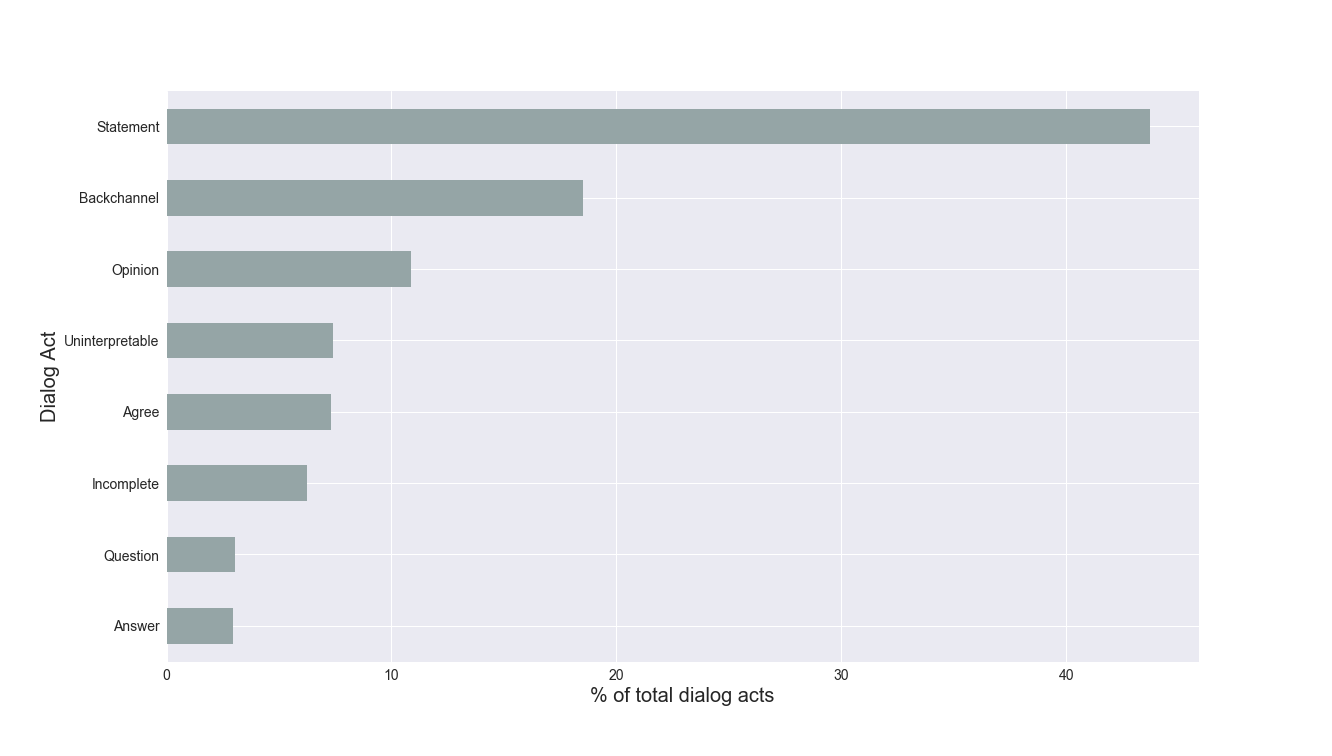
\includegraphics[width=\textwidth]{../scikitlearn/figures/f1.png}
 \caption{Dialog act relative count\label{overflow}}
 \label{f1}
 \end{figure}

Next we wanted to measure the correlation between dialog act type and the probability of a turn change.  In figure \ref{f2}, each bar measures the number of time a turn change occurred after a dialog act type divided by the total dialog act of this type. Or the probability that a dialog act of the said type will lead to turn change. We observe that the majority of back channels and question (which are usually the first utterance in an question-answer adjacency pair) will lead to a turn change.

\begin{figure}[ht!]
\centering
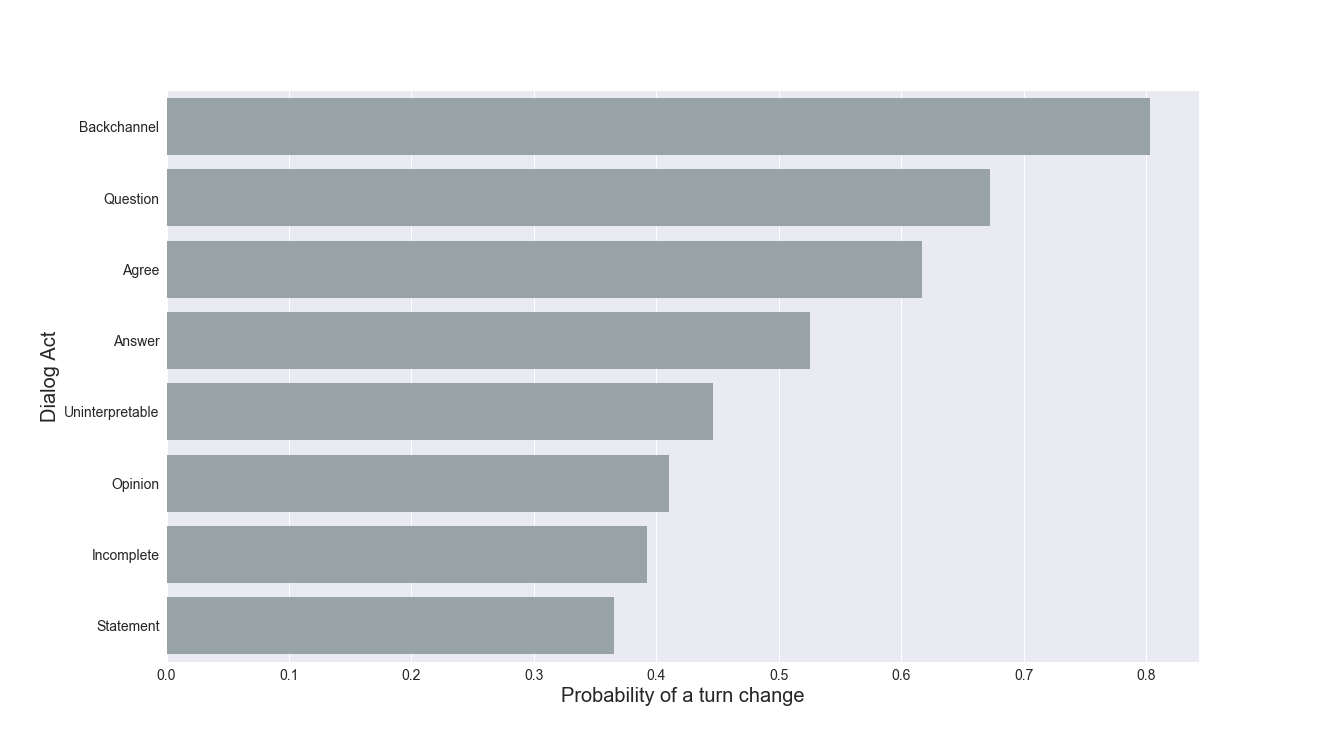
\includegraphics[width=\textwidth]{../scikitlearn/figures/f2.png}
\caption{Dialog act probability of turn change\label{overflow}}
\label{f2}
\end{figure}
\pagebreak 